\documentclass[tikz]{standalone}

\usepackage{color}

\usetikzlibrary{math,decorations.pathreplacing,calc,decorations.markings}

\tikzset{->-/.style={decoration={
			markings,
			mark=at position {0.5*\pgfdecoratedpathlength+.5*3pt} with {\arrow{>}}},postaction={decorate}}}

\tikzset{-<-/.style={decoration={
			markings,
			mark=at position {0.5*\pgfdecoratedpathlength+.5*3pt} with {\arrow{<}}},postaction={decorate}}}

\begin{document}
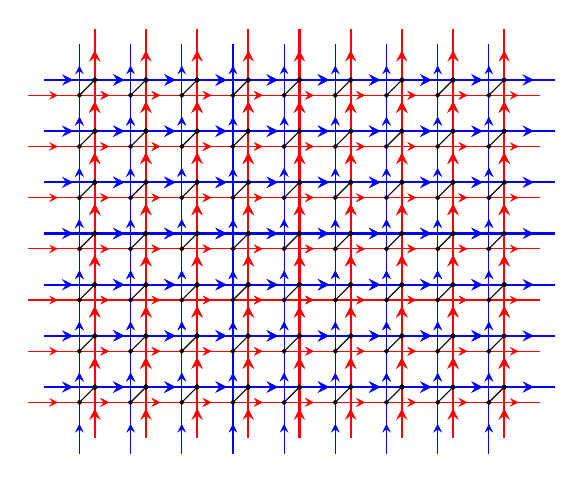
\begin{tikzpicture}[every node/.style={draw,shape=circle,minimum size=.5mm,inner sep=0pt,outer sep=0pt,fill=black},>=stealth, scale=0.65]
\foreach \i in {-4,...,4} {
	\foreach \j in {-3,...,3} {
		\draw[->-,red] (\i,\j) -- ({\i+1},{\j});
		\draw[->-,red] ({\i-1},\j) -- (\i,\j);
		
		\draw[->-,blue] (\i,\j) -- ({\i},{\j+1});
		\draw[->-,blue] (\i,{\j-1}) -- (\i,\j);
	};
};
\foreach \i in {-4,...,4} {
	\foreach \j in {-3,...,3} {
		\node () at ($(\i,\j)$) {};
	};
};

\foreach \i in {-4,...,4} {
	\foreach \j in {-3,...,3} {
		\draw[->-,red,thick] (\i+0.3,\j+0.3) -- ({\i+0.3},{\j+1+0.3});
		\draw[->-,red,thick] (\i+0.3,{\j-1+0.3}) -- (\i+0.3,\j+0.3);
		
		\draw[->-,blue,thick] (\i+0.3,\j+0.3) -- ({\i+1+0.3},{\j+0.3});
		\draw[->-,blue,thick] ({\i-1+0.3},\j+0.3) -- (\i+0.3,\j+0.3);
		
		\draw [] (\i,\j) -- (\i+0.3,\j+0.3);
	};
	\foreach \i in {-4,...,4} {
		\foreach \j in {-3,...,3} {
			\node () at ($(\i+0.3,\j+0.3)$) {};
		};
	};
};	

\end{tikzpicture}

	
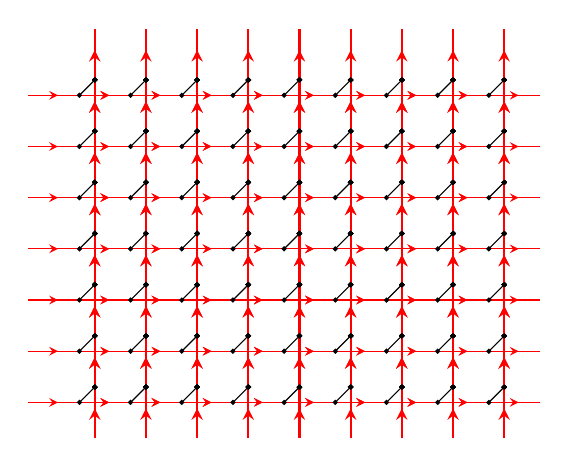
\begin{tikzpicture}[every node/.style={draw,shape=circle,minimum size=.5mm,inner sep=0pt,outer sep=0pt,fill=black},>=stealth, scale=0.65]
\foreach \i in {-4,...,4} {
	\foreach \j in {-3,...,3} {
		\draw[->-,red] (\i,\j) -- ({\i+1},{\j});
		\draw[->-,red] ({\i-1},\j) -- (\i,\j);
	};
};
\foreach \i in {-4,...,4} {
	\foreach \j in {-3,...,3} {
		\node () at ($(\i,\j)$) {};
	};
};

\foreach \i in {-4,...,4} {
	\foreach \j in {-3,...,3} {
		\draw[->-,red,thick] (\i+0.3,\j+0.3) -- ({\i+0.3},{\j+1+0.3});
		\draw[->-,red,thick] (\i+0.3,{\j-1+0.3}) -- (\i+0.3,\j+0.3);
		
		\draw [] (\i,\j) -- (\i+0.3,\j+0.3);
	};
	\foreach \i in {-4,...,4} {
		\foreach \j in {-3,...,3} {
			\node () at ($(\i+0.3,\j+0.3)$) {};
		};
	};
};	

\end{tikzpicture}
\end{document}
